\section{Datalag}

\subsection{DAL}

\begin{frame}{DAL --- Data Access Layer}
  \framesubtitle{Overblik}
  \begin{itemize}
    \item Interface versus Implementation
    \item CRUD
    \begin{itemize}
      \item \texttt{{\Large C}reate}
      \item \texttt{{\Large R}etrieve}
      \item \texttt{{\Large U}pdate}
      \item \texttt{{\Large D}elete}
    \end{itemize}
  \end{itemize}
\end{frame}

\begin{frame}{DAL --- Data Access Layer}
  \framesubtitle{Databaserelationer}
  \begin{itemize}
    \item One--to--one
    \item One--to--many
    \item Many--to--many
  \end{itemize}
\end{frame}


\subsection{Modellag}

\begin{frame}{Modellag}
  \framesubtitle{UML--diagram}
  \begin{center}
    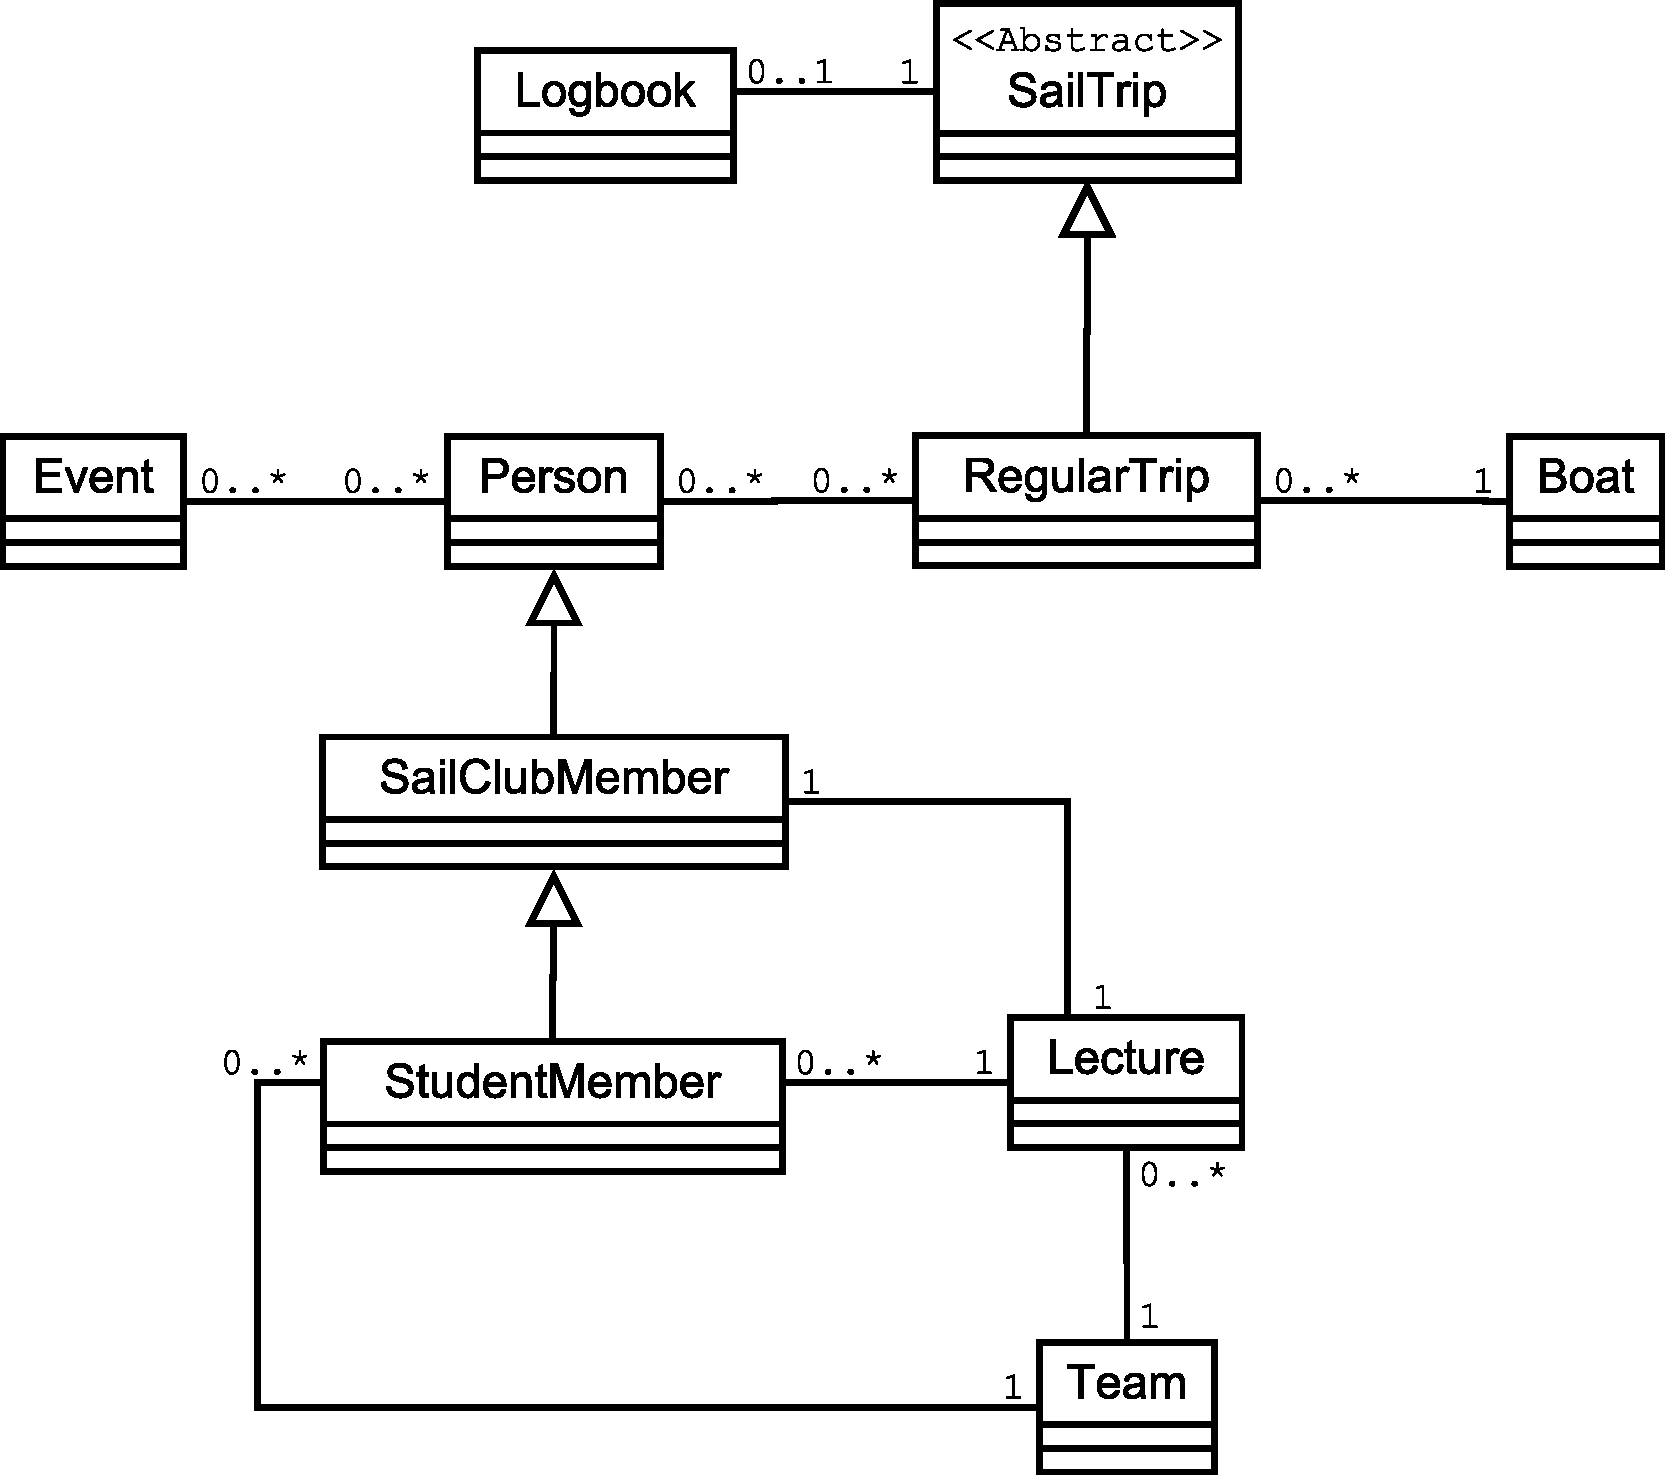
\includegraphics[width=0.8\textwidth,height=0.8\textheight,keepaspectratio]{images/UML.pdf}
  \end{center}
\end{frame}

\begin{frame}{Modellag --- Relationer}
  \framesubtitle{One--to--one}
  \begin{center}
    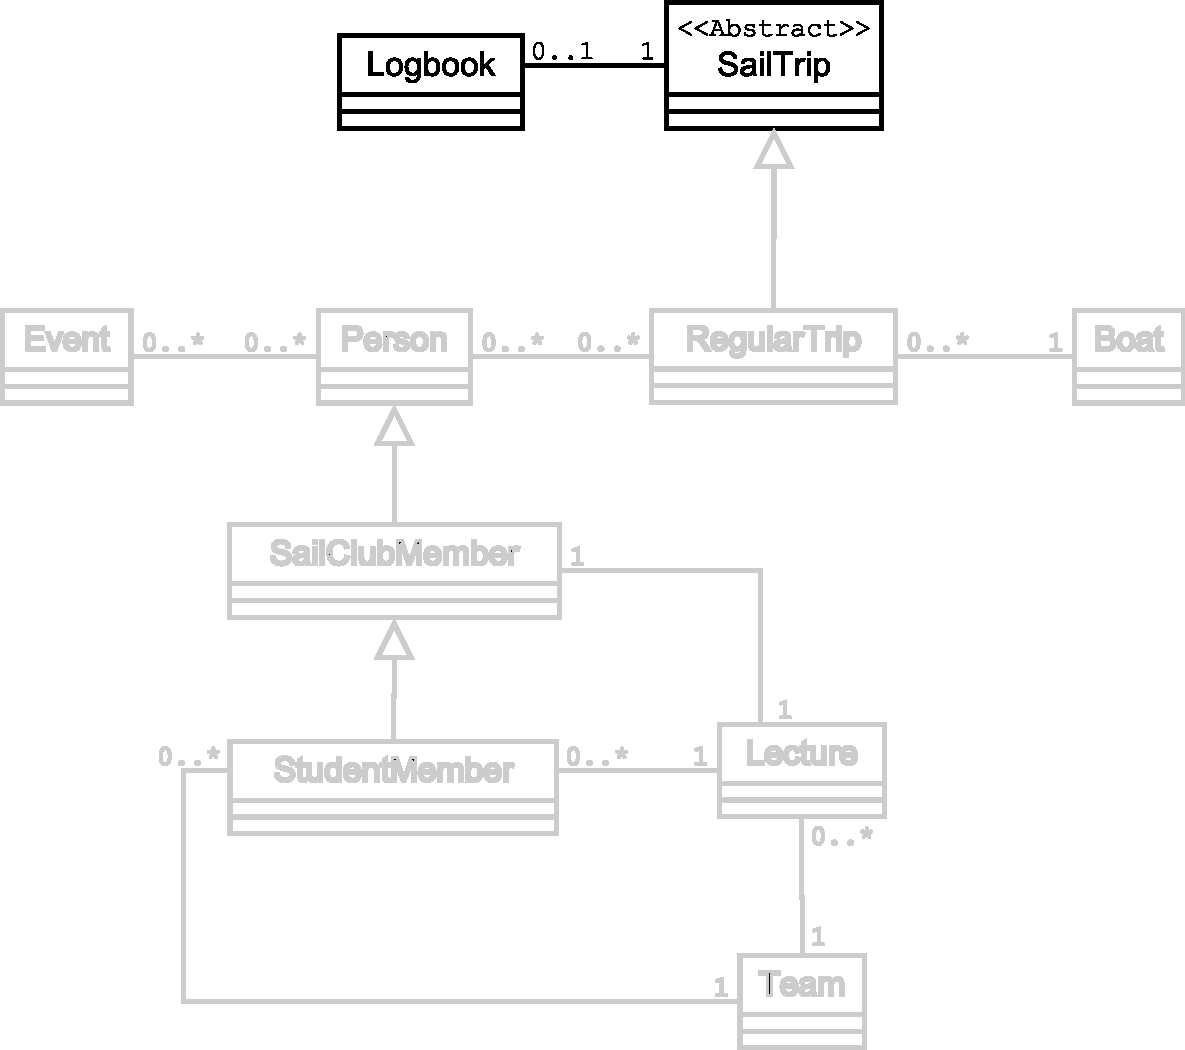
\includegraphics[width=0.8\textwidth,height=0.8\textheight,keepaspectratio]{images/One-to-one.pdf}
  \end{center}
\end{frame}

\begin{frame}{Modellag --- Relationer}
  \framesubtitle{One--to--many}
  \begin{center}
    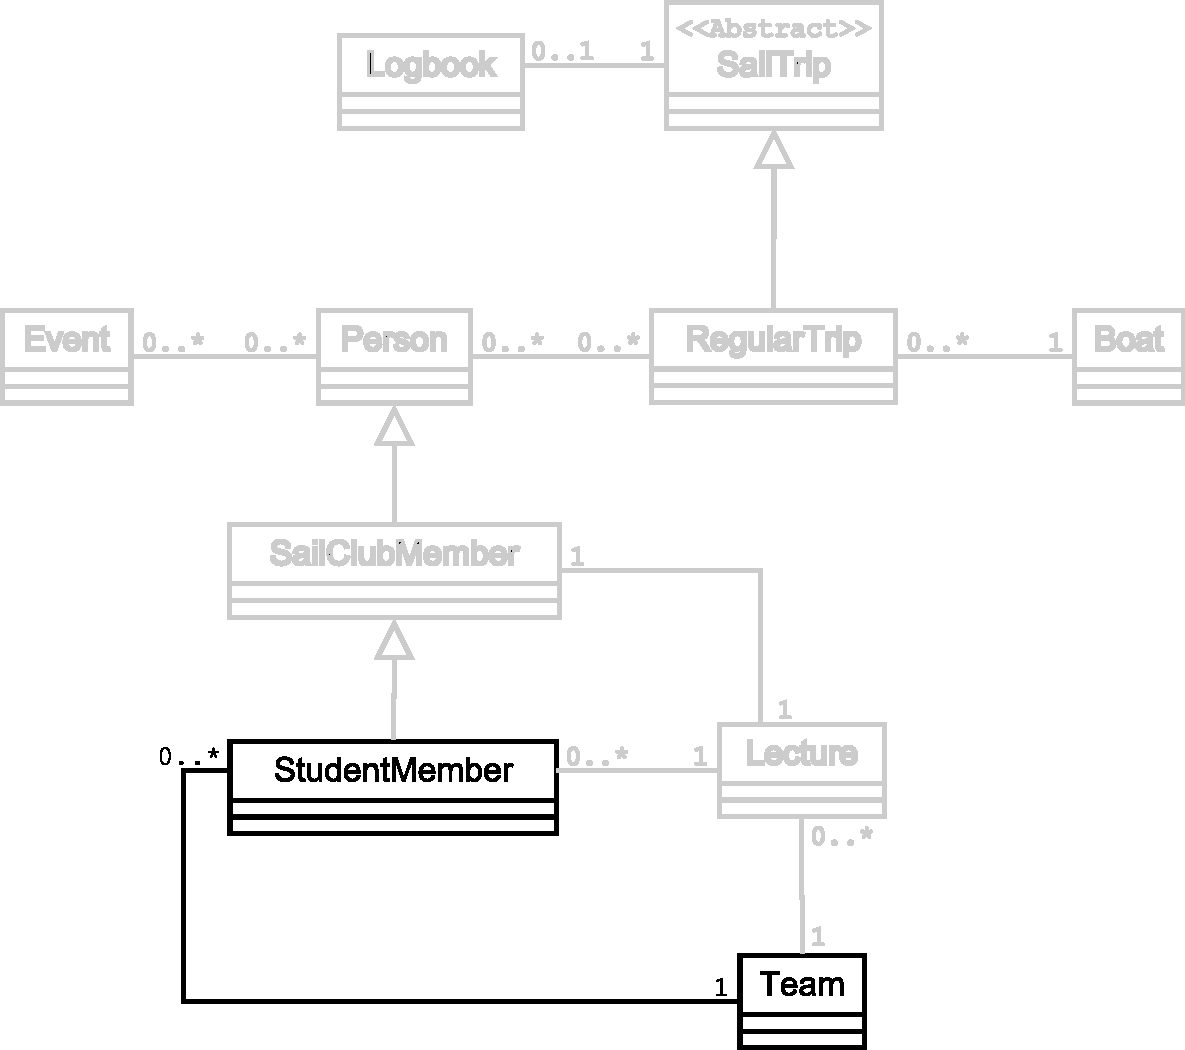
\includegraphics[width=0.8\textwidth,height=0.8\textheight,keepaspectratio]{images/One-to-many.pdf}
  \end{center}
\end{frame}

\begin{frame}{Modellag --- Relationer}
  \framesubtitle{Many--to--many}
  \begin{center}
    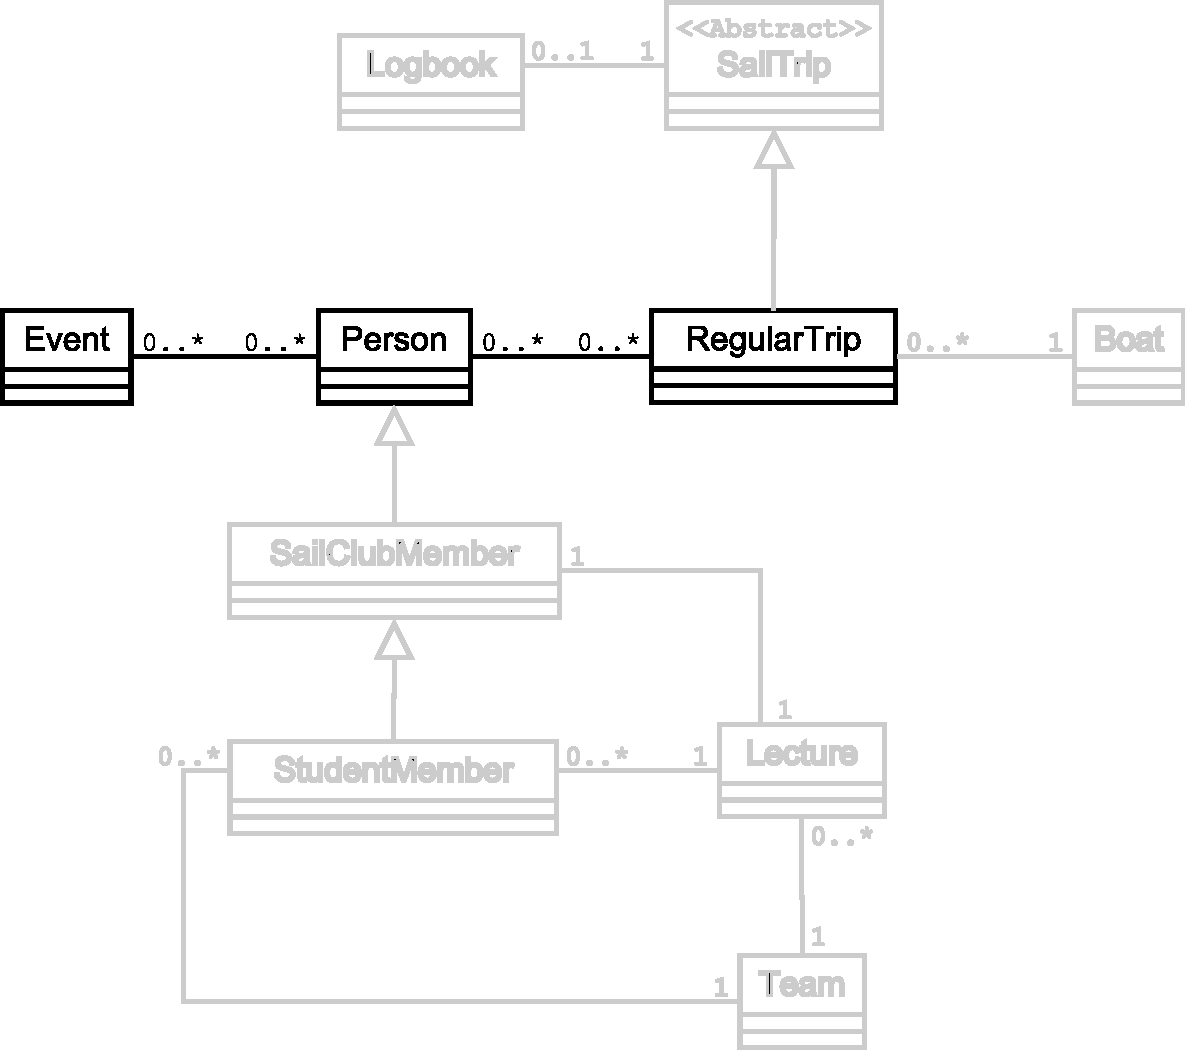
\includegraphics[width=0.8\textwidth,height=0.8\textheight,keepaspectratio]{images/Many-to-many.pdf}
  \end{center}
\end{frame}


\subsection{Persistenslag}

\begin{frame}{Persistenslag}
  \framesubtitle{Entity Framework --- Code First}
  \onslide<1>{%
    \begin{beamerboxesrounded}[upper=headerCol,lower=bodyCol,shadow=true]{Fordele}
      \begin{itemize}
        \item Isolering af databaselogik (SQL--forespørgsler)
        \item POCO (Plain Old CLR Objects)
        \item RAD (Rapid Application Development)
      \end{itemize}
    \end{beamerboxesrounded}%
  }
  \onslide<2>{%
    \begin{beamerboxesrounded}[upper=headerCol,lower=bodyCol,shadow=true]{Ulemper}
      \begin{itemize}
        \item Migrations
        \item Data annotations
      \end{itemize}
    \end{beamerboxesrounded}%
  }
  \onslide<3>{%
    \begin{beamerboxesrounded}[upper=headerCol,lower=bodyCol,shadow=true]{Forhindringer}
      \begin{itemize}
        \item Context levetid
      \end{itemize}
    \end{beamerboxesrounded}%
  }
\end{frame}

\begin{frame}{Persistenslag}
  \framesubtitle{SQLite}
  \onslide<1>{%
    \begin{beamerboxesrounded}[upper=headerCol,lower=bodyCol,shadow=true]{Fordele}
      \begin{itemize}
        \item God kompatibilitet med CRUD.
        \begin{description}
          \item[Create] \texttt{INSERT}
          \item[Retrieve] \texttt{SELECT}
          \item[Update] \texttt{UPDATE}
          \item[Delete] \texttt{DELETE}
        \end{description}
        \item Fuld kontrol over det underliggende.
      \end{itemize}
    \end{beamerboxesrounded}%
  }
  \onslide<2>{%
    \begin{beamerboxesrounded}[upper=headerCol,lower=bodyCol,shadow=true]{Ulemper}
      \begin{itemize}
        \item Kræver kendskab til SQL.
        \item Komplekse relationer kan være svære.
      \end{itemize}
    \end{beamerboxesrounded}%
  }
  \onslide<3>{%
    \begin{beamerboxesrounded}[upper=headerCol,lower=bodyCol,shadow=true]{Forhindringer}
      \begin{itemize}
        \item Enkeltbrugersystem --- Ikke thread--safe.
        \begin{itemize}
          \item ''Database is locked``
        \end{itemize}
      \end{itemize}
    \end{beamerboxesrounded}%
  }
\end{frame}

\begin{frame}{Persistenslag}
  \framesubtitle{Mock--data med persistens}
  \onslide<1>{%
    \begin{beamerboxesrounded}[upper=headerCol,lower=bodyCol,shadow=true]{Fordele}
      \begin{itemize}
        \item Nødløsning --- Ikke oprindeligt et persistenslag.
        \item Hurtigt --- Hukommelsesbaseret.
      \end{itemize}
    \end{beamerboxesrounded}%
  }
  \onslide<2>{%
    \begin{beamerboxesrounded}[upper=headerCol,lower=bodyCol,shadow=true]{Ulemper}
      \begin{itemize}
        \item Ikke skalerbart.
        \item Risiko for datatab.
      \end{itemize}
    \end{beamerboxesrounded}%
  }
\end{frame}